\documentclass[conference,compsoc,hidelinks]{IEEEtran}
\usepackage[utf8]{inputenc}
%\usepackage{hyperref}
\usepackage{lipsum}
\usepackage{graphicx}
\usepackage[pdftex,
pdfauthor={Rene Kremer},
pdftitle={An Overview and Comparison of State of the Art Methodologies for the upcoming challenges of industrial digitization},
pdfsubject={Overview and Comparison of Architectures like PERFoRM and PRIME in the field of industrial revolution},
pdfkeywords={System Architecture, Seamless System Reconfiguration, Multi Agent System, Industrial Revolution, Industrial Digitization},
pdfproducer={PDFLatex},
pdfcreator={PDFLatex}]{hyperref}

% *** CITATION PACKAGES ***
%
\ifCLASSOPTIONcompsoc
  % IEEE Computer Society needs nocompress option
  % requires cite.sty v4.0 or later (November 2003)
  \usepackage[nocompress]{cite}
\else
  % normal IEEE
  \usepackage{cite}
\fi

% *** GRAPHICS RELATED PACKAGES ***
%
\ifCLASSINFOpdf
\else
\fi
% correct bad hyphenation here
\hyphenation{op-tical net-works semi-conduc-tor ana-ly-tics}


\begin{document}

\title{An Overview and Comparison of State of the Art Methodologies for the upcoming challenges of industrial digitization}

\author{\IEEEauthorblockN{René Kremer}
\IEEEauthorblockA{University of Lübeck\\
%Institute of Computer Engineering\\
Lübeck, Germany\\
Email: rene.kremer@student.uni-luebeck.de}}

% make the title area
\maketitle

\begin{abstract}
Driven by the fourth industrial revolution emerges a need for concepts, methods and technologies which will take on the new challenge of digitalization. In future systems digitalization is an important principle with the goal of processing and collecting large amounts of data as well as having smart, pluggable, cooperating and collaborating components. A special design process has to be addressed to allow building evolvable and complex systems for various requirements and use cases \cite{Peres2017}. This paper focuses on architectures like PERFoRM and the PRIME Framework for Multi Agent Systems (MAS) by comparing them, as both are trying to support the new upcoming system designs.
\end{abstract}

\section{Introduction} % first page
% no \IEEEPARstart
The world wide trend for globalization pressures the manufacturing domain. Especially Europe is pressured by constantly rising US and Asian competitors. This leads to customers being able to order from foreign companies and products eventually being more customized, cheaper and with higher quality. This circumstance drives manufacturing companies to find solutions to keep up with these changes \cite{HarmonizedSystems}. 

While striving for ways to reduce production costs and raise quality of products, another factor to the company performance are disturbances like delays, shortages from suppliers or resource breakdowns. These disturbances can have a deep impact on the performance and might lead to losing customers. This world-market reshape raises the urge to develop new manufacturing paradigms, new manufacturing control systems and smarter manufacturing equipment with features such as modularity, reconfigurability and flexibility \cite{SCHEIFELE2014398} to enable a complete process integration. The underlying basis for this integration is production digitization, massive information exchange and processing. 

The use of Internet of Things (IoT) allows for collection of massive sensorial data, which can be processed by Big data techniques. This allows production resources to become smarter, pluggable and distributed. The design of production systems shifts from traditional monolithic hierarchical systems into a distributed and horizontal structure, where heterogeneous components are cooperating and collaborating with another. A common paradigm to reach such a structure is called Cyber-Physical-System (CPS), where the physical (real world) and logical part (cyber world) are merged \cite{SpecPERFoRM}.

National and transnational programs emerged to support research on these scientific and technological areas. These programs strive to solve the problems of the industrial revolution are called: "Industrie 4.0" in Germany, "Made in Sweden 2030" in Sweden, "La Nouvelle France Industrielle" in France, "Smart Industry" in Netherlands, "Industria Conectada 4.0" in Spain, "Innovate UK" in United Kingdom and "Fabbrica Intelligente" in Italy \cite{SpecPERFoRM}. 

The European commission, industry and research institutes are trying to solve these new problems and issues, but only few brought successful solutions into industrial applications. Many projects focus on solving specific problems but neglect other technological issues. Research projects are often using non-standardized interfaces and platforms, which aren't yet applied in industry. 

Some projects showed that Multi-Agent Systems (MAS) provide a distributed intelligence to the components of the system while Service-oriented Architecture (SoA) provide plugability and also vertical and horizontal system integration \cite{Colombo2009}. Ontologies are needed to define a common data model for communication and data processing \cite{Peres2017}.

The FP7 PRIME project, funded by the EU, developed an agent based architecture, which will be topic of \autoref{sec:PRIME}, to allow semi-automatical reconfiguration through aggregating and compositing skills in combination with a Human Machine Interface Agent (HMIA). The HMIA works as a gateway user interface providing different system users, system configurations and specifications. PRIME shows how reconfiguration by parametrization can be done using MAS.

The PERFoRM project, which will be introduced in \autoref{sec:PERFoRM}, combines existing solutions of successful public and private research projects into one common platform to make an industrial adoption possible \cite{HarmonizedSystems}. PERFoRM aims to develop an approach to integrate legacy systems through adapters, allow seamless production system reconfiguration through the plug-and-produce concept as well as human interactions, but also to provide advanced tools like intelligent decision support, scheduling and simulation to aid the system \cite{SpecPERFoRM}.

This report gives an overview of state of the art technologies addressing the issues of the industrial revolution 4.0 and compares the PRIME architecture with the PERFoRM architecture, which aim to provide solutions for these new cyber-physical-production-systems (CPPS).


%\hfill rk

%\hfill Juni 15, 2017

% no keywords

\IEEEpeerreviewmaketitle

\section{State of the Art Methodologies} \label{sec:state-of-the-art}% second page
In this section different approaches will be introduced, which are the results of successful projects. 

\subsection{Multi-Agent Systems}
Multi-Agent Systems (MAS) are an approach to develop an agent based decentralized control architecture for production systems. This allows an easy support for cyber-physical concepts and the creation of smart components as agents in the system. This means the production system is a collection of agents, where agents interact with each other. Every agent got an own action scope and is aware of the status of its surrounding agents. Therefore it is possible for them to self-organize in case of changes and disturbances, which means they reconfigure and operate accordingly to its environment \cite{HarmonizedSystems,Peres2017}.

\subsection{Plug and Produce Technology}
"Plug and Produce" technologies try to build modules, which can integrate intelligent components. This is accomplished by using standard interfaces and adapters for existing interfaces. Following this approach it is possible to use plug-and-produce devices, which could have built-in intelligence and profit of sensors and actors. These plug-and-produce devices might be used to integrate new capabilities to an existing production systems or a new one \cite{HarmonizedSystems}. Self*-Features possess an important role in these upcoming architectures \cite{SpecPERFoRM} and the "Plug and Produce" technology should focus on self-adaptive and reconfigurable components to support a flexible solution. MAS was used in some projects to accomplish plug-and-produce with self-adaption. PRIME, which was developed in scope of the PRIME project and funded by the European FP7 program, used a MAS in this context to support semi-automatical configuration through a human-machine-interface (HMI). Reconfiguration in the PRIME architecture is handled through different agent roles and enables the integration of legacy systems \cite{HarmonizedSystems}.

\subsection{Service-oriented Architecture}
Other projects researched the possible use of Service-oriented Architectures (SoA), which are mostly commonly used in the context of Web services. The principle of SoA could be used at a device and application level to enable and integrate distributed smart embedded systems \cite{Colombo2009}. These components are handled as services, which are flexible parts in this kind of architecture. Therefore it is important to create an open and flexible environment that is extended by the scope of the collaborative SoA \cite{HarmonizedSystems}. This means that the industrial middleware needs to be able to discover and register new services and also expose functionalities of the heterogeneous components as services \cite{SpecPERFoRM}. Data transformation for these different services also needs to be handled by the middleware, which adds additional intelligence to this component. Once the groundwork is done, integration of new services and communication between existing ones can be simplified on different levels of the enterprise architecture. As services are interoperable and reusable this approach allows to develop self-learning production systems by using data mining and context awareness \cite{HarmonizedSystems, DENKENA2014406, Peres2017}.


\subsection{Cloud Technology}
Towards the goal of developing an architecture that can be used in the context of industry 4.0 and its digitalization, the possible use of cloud technologies was investigated. Cloud technologies are used to build a common data model to integrate data of heterogeneous components together onto one platform. This allows the creation of a systematic knowledge generation ranging from design till usage phase by knowledge gathering and refining. Some projects even showed that SoA and Cloud technologies work hand in hand \cite{HarmonizedSystems}.  

\subsection{Conclusion}
Different solutions were developed for the new agile-manufacturing generation using agent-systems, (smart) component networks, service-oriented paradigms and cloud principles to overcome the challenges of the migration from traditional production systems towards cyber-physical-production-systems (CPPS) \cite{HarmonizedSystems}.

1. Integration: The problem posed by each of these solutions is the individual integration of existing components and legacy systems. Therefore a common interface and standard needs to be established for a wide use in different industries.

2. Support Businesses: It is not enough to develop new concepts and technologies if it is not benefiting the goal of businesses. Requirements and performance indicators needs to be analyzed to support those real business requirements and therefore improve the overall performance of the business.

3. Human Factor:  The human factor is a flexibility driver and therefore needs special attention \cite{Colombo2009}. Not only highly usable HMIs need to be developed. The impact of these upcoming concepts and architectures needs to be analyzed and evaluated. Necessary skills for operators and maintainers possibly will change. Activities on education and training become important parts so that human workers can keep up with new state of the art procedures and technologies.

4. Maturity and Migration: These new approaches, which are currently state of the art, are not fully tested in industry. As the migration of new technologies will have a big impact on the production and expenses of a company a good and tested migration strategy needs to be developed. Special attention lies on the smooth integration of legacy systems.

\section{PRIME} \label{sec:PRIME}% third page

This section briefly introduces the PRIME architecture based on the agents this architecture uses in its MAS.
\subsection{Motivation}
PRIME provides an architecture using agent technology, which might lead to time processing issues in terms of communication and process control. However, PRIME uses a hybrid structure integrating a MAS with traditional automation equipment (programmable logic controllers). In this context the control system of the production system should operate independently to the MAS and offer more flexibility to the overall system. This is achieved by providing an easy and seamless reconfiguration of the control system, which is handled by the MAS \cite{Hybrid}.

\subsection{Architecture}
The architecture uses a data base to store templates of the products, composition rules and system skills. System skills are software abstractions of physical modules, which are abstracted as Component Agents (CA), and processes. Skills include information such as configuration and parameters and can be aggregated as a combination of different skills of CAs \cite{Hybrid}.

\begin{figure}[ht]
	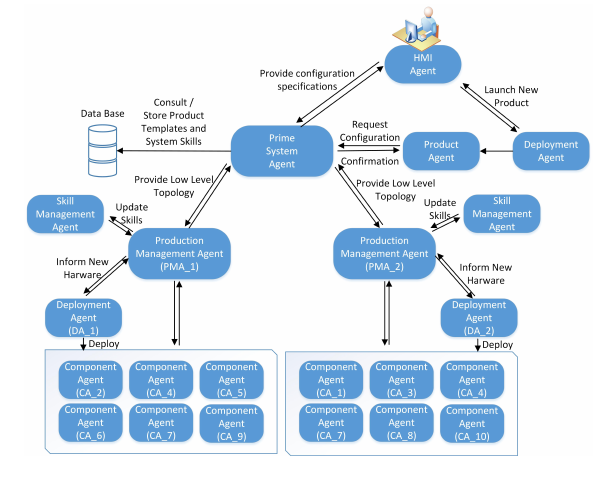
\includegraphics[width=\columnwidth]{img/PRIME-Architecture.png}
	\caption{PRIME Architecture \cite{Hybrid}}
	\label{fig:prime-architecture}
\end{figure}
\noindent
As previously mentioned PRIME is agent based and uses 7 different types of agents:

1. Component Agent (CA): Already mentioned, the CA represents system components, i.e. hardware, physical devices etc., and includes interaction logic required for reconfiguration of its physical component. CAs contain the previously mentioned skills \cite{Hybrid}.

2. Human Machine Interface Agent (HMIA): This agent works as a (gateway) user interface to allow different system users to have a view on the systems state and interact with it as seen in \autoref{fig:prime-architecture}.

3. Prime System Agent (PSA): System creation starts with system users interacting with the PSA (mediated by the HMIA). The PSA also is connected to a data base holding all information on product templates and system skills. With this knowledge it controls and connects to the production management agents (PMA). On a change of skill sets the PSA is the last informed instance and stores these updates in the knowledge data base. After storing the new composition rules for the skill sets, it down-streams them to all connected PMAs to update their skills. If a new Product Agent (PA) is launched, and therefore another product introduced to the system, the PSA verifies if the requirements for the new product can be met with the existing skill sets. If that is the case, the PMAs for theses skill sets will be re-parametrized and in the end forward the new parameters to the CAs \cite{Hybrid}.

4. Deployment Agent (DA): The DA is responsible for launching all agents. Therefore it is assumed that all controllers, where the infrastructure will be deployed, have a running DA. Using local validation rules the DA asserts if an agent of a specific class can be launched in the controller \cite{Hybrid}. 

5. Production Management Agent (PMA): After setting up and creating the system, PMAs will be started. A PMA abstracts a subsystem and therefore is an aggregation of subsystems and/or system components. As shown in \autoref{fig:pma-tree} a PMA can include other PMAs as part of its subsystem. The last level of this PMA-Tree consists of CAs to connect to physical modules (as previously mentioned).  A PMA is associated to one Skill Management Agent (SMA) and responsible to launch it. 

\begin{figure}[ht]
	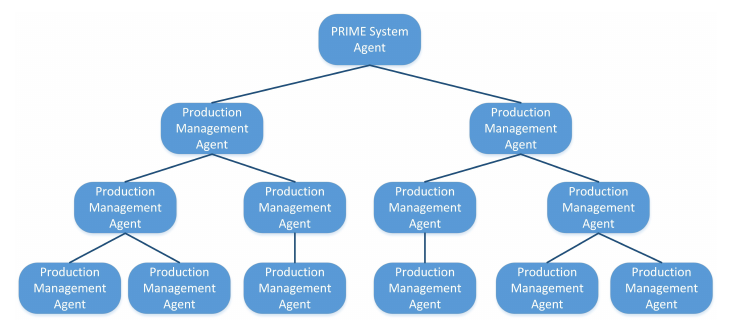
\includegraphics[width=\columnwidth]{img/Production-Management-Agent-Tree.png}
	\caption{Production Management Agent tree \cite{Hybrid}}
	\label{fig:pma-tree}
\end{figure}

Every time the set of agents changes, the PMA needs to verify if agents are leaving or joining the sub system and forward that information up to its parent PMA or even the PSA (in case of a top level PMA). For joining agents the PMA has to validate if they can operate in the new context and also if they change the number and type of skills the PMAs subsystem can provide. In case the PMA gets updates from its parent PMA or PSA it forwards these composition rule updates to its SMA and subordinate PMAs. This change of rules and skills will only be processed if the PMA receives an inform message that confirms the successful update of higher-level agents. Therefore updating is a cascading process and atomic, which means that the entire system is updated or the update does not become effective. This mechanism keeps the integrity and consistency of the reconfiguration information for the system \cite{Hybrid}.

6. Skill Management Agent (SMA): As previously mentioned a PMA has a SMA holding the topological information about the subsystem and its skill composition/aggregation rules. These skills are reconfigurable as the SMAs are a virtual representation of these skills. In case of changes, SMAs work parallel, save new rules and verify changes of existing skills while the PMA updates the topological structure. This asynchronous behavior is important for bigger systems, which have many skill composition rules that may take longer to compute \cite{Hybrid}.

7. Product Agent (PA): Whenever a new product is introduced to the system a new instance of a PA is created. PAs hold all information that describe the new product e.g. process plan and associated skills. The specification of the product will be sent to the PSA as well as the process requirements, which verifies if the system can meet those requirements \cite{Hybrid}. 

\section{PERFoRM} \label{sec:PERFoRM} % fourth page
This section gives a brief introduction to another architecture called PERFoRM, its motivation, assumptions and architectural elements.

\subsection{Motivation}
The PERFoRM project is funded by the European Unions Horizon 2020 research and innovation programme and investigates the requirements for new innovative production systems. PERFoRM does not try to develop a new architecture from scratch but instead tries to re-use the results of previous successful projects in this field \cite{SpecPERFoRM}. 

\subsection{Assumptions}
1. Integration of legacy systems: As most of the industry uses legacy systems the integration of these systems is an important part to consider. Standard interfaces for syntax and semantic define how to communicate with components of the system. Technology adapters connect existing components to these interfaces. Once these interfaces and adapters are commonly established heterogeneous components can be connected to the communication infrastructure, which can address other backbone level systems via Machine-to-Machine (M2M) and Enterprise-Service-Bus (ESB) technologies.

2. Integration of advanced planning and simulation applications: New CPPS are based on smart components. To support smart and self*-features of those devices it is essential to allow simulation and planning. This allows them to be agile and adaptive to its surroundings. A way to enable this is using MAS and cloud technologies to propagate strategies and decision making.

3. Seamless data representation: Keeping in mind that devices are mostly heterogeneous different representations of data need to be processed. An standard representation of industrial data models and gateways for data transformation on machinery and backbone level are needed to accomplish this problem.

4. Components and Configuration on the fly: Disturbances of the work-flow need to be recognized and handled. Distributed approaches, e.g. MAS or SoA, combined with registry and discovery mechanisms enable the architecture to support a plug-and-play approach for components. In case of disturbances, planned or not, e.g. maintenance or device failure, reconfiguration of running components might be necessary. Other projects, like PRIME, showed concepts to support reconfiguration and also self*-features in an productive environment.

5. Distributed and heterogeneous components: In addition to the previously mentioned standard interfaces and technology adapters, service-oriented design principles like SoA allow a more abstract view on distributed and heterogeneous components. The system can expose functionalities as services as well as aggregate and composite those services. Therefore the combination of services can create new services and also describe services used for self-organization of smart components in the production system.

6. Intelligent production components: Components getting more powerful in terms of performance allow for decentralized intelligence. Artificial Intelligence methods, e.g. MAS, could be supported by these components. Data analysis could be handled on an advanced level to help the AI and their self*-features. An example would be the self-adaption in case a surrounding component fails. As these smart devices watch their surroundings and the status of other devices they can react to changes based on status or disturbances in another part of the work-flow.

7. Integrate Humans: Even with all those smart devices and innovative ways to enhance new performance peaks to satisfy customer needs, humans still play an important role in operating and maintaining these systems. With changing techniques and concepts human operators and maintainers need to adapt to those changes. HMI and mobile applications need to be highly usable and supportive. Education and Training activities need to take new ways to keep up with these upcoming technologies and enable humans to understand, operate and maintain them \cite{SpecPERFoRM}.

\subsection{Architectural Elements}
Based on the assumptions made by PERFoRM there are elements in the architecture which are deemed necessary.

The integration of legacy systems and communication between distributed heterogeneous components make standard interfaces and technology adapters essential.
Therefore standards for these interfaces and adapters need to be established so that regardless of the manufacturers of devices and software components it is ensured that they fit into the architecture.

\begin{figure}[ht]
	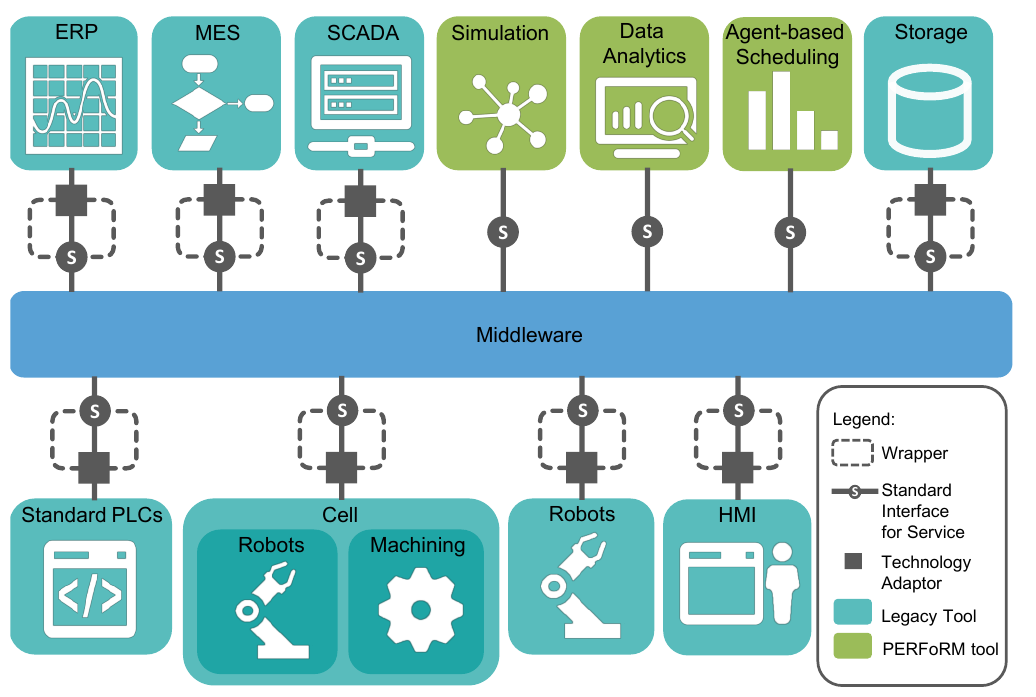
\includegraphics[width=\columnwidth]{img/PERFoRM-Architecture.png}
	\caption{The PERFoRM system architecture\cite{SpecPERFoRM}}
	\label{fig:PERFoRM-Architecture}
\end{figure}

As seen in \autoref{fig:PERFoRM-Architecture} another important part of the architecture is the industrial middleware. To ensure seamless data representation, data transformation and approaches like MAS a smart middleware is necessary. In terms of service-orientation these features are enriched with service registry and discovery. Depending on the chosen architecture design the middleware might be the central communication and organization hub for all other parts of the system.

\section{Comparison} \label{sec:comparison} % fifth to sixth page
This sections compares PRIME with PERFoRM as far as it is possible. Both architectures are in different maturity phases and serve different purposes and motivations.

\subsection{Motivation and Purpose}
As mentioned in \autoref{sec:PRIME}, PRIME targets the seamless reconfiguration of production components using a hybrid system powered by a MAS and therefore tries to reduce setup time and non value-adding activities. It focuses on the lower level of production and industrial systems. In terms of ISA-95 layers it handles level 2, which is supervisory control. The other levels are physical processes (L0), automation control (L1), manufacturing operations management (L3) and business planning and logistics (L4)  \cite{SpecPERFoRM}.

PERFoRM on the other hand tries to provide an architecture for all of the described layers. Compared  to the FP7 program, Horizon 2020 is currently active i.e. PERFoRM can use the insight gained by the PRIME project (and many others) in its specification \cite{SpecPERFoRM}. The potential of PERFoRM is not fully researched and as shown in \autoref{sec:PERFoRM} the specification makes some assumptions about future systems and tries to handle heterogeneous system components, legacy systems and different industrial domains equally well.

\subsection{Seamless reconfiguration}
PRIME shows that using a MAS can provide an architecture that is ready to tackle the challenge of seamless integration \cite{Hybrid}. Further research needs to be done to prove that it handles reconfiguration well on a bigger scaled shop floor. The test cases in \cite{Hybrid} provide a glimpse of the needed time for the reconfiguration. As it is a product of the FP7 PRIME project, a research funding program active from 2007 to 2013, it seems more like a short term solution to the whole issue of digitization. The abstraction of component sets as subsystems by a PMA is a good way to get a clear topological structure and avoid creating bottlenecks by utilizing their vertical and horizontal scalability. On the other hand this abstraction of subsystems can prove to be a disadvantage. If one PMA fails, the whole subsystem of this PMA is cut off the architecture. The same goes for the PSA. A backup plan should be devised to counter the occurrence of this problem. As such, a heartbeat algorithm for example could check on dead agents, trigger a reboot for dead agents or even a transfer process mapping the children of the failed PMA to another PMA for a short amount of time. The test cases used in \cite{Hybrid} show that plugging and unplugging components is registered and processed in under a second. Therefore this might be a short term fix for failures.

PERFoRM takes on the assumptions that there is a need for plug and play of production, components and reconfiguration on the fly and suggests distributed technologies e.g. MAS or SoA. Furthermore it assumes that some production components can be enriched with intelligence using AI methods in combination with MAS \cite{SpecPERFoRM}. As PRIME showed how to integrate logic for reconfiguration PERFoRM might adopt this approach to fulfill the assumed requirements. Seamless reconfiguration is identified as a requirement but there is no final solution on how to reach this goal. If PRIMEs seamless reconfiguration solution will be adopted, it needs to be checked if the whole agent-based architecture described by PRIME is part of the intelligence industrial middleware. Alternatively, it could be a combination of new PERFoRM Tools and middleware or a single new tool like \emph{Agent-based Scheduling} as shown in \autoref{fig:PERFoRM-Architecture}. 

\subsection{Integration of existing systems}
Many companies are using legacy systems as well as legacy components \cite{HarmonizedSystems}. New architectures need to support the integration of those systems and components as changing all software and hardware components is not an option. PRIMEs component agents are responsible for handling the communication, parametrization and configuration of the physical components \cite{Hybrid}. They interface those components and provide a interaction logic to reconfigure the connected devices. 

PERFoRMs goal is to integrate many heterogeneous hardware and software components using a smart middleware as shown in \autoref{fig:PERFoRM-Architecture}. For this purpose PERFoRM introduces standard interfaces for each component so that the middleware can call functionalities of the component using a common interface \cite{SpecPERFoRM}. The standard interface uses a technology adapter which handles the connection and communication to and with the component. By doing this, heterogeneous devices and systems can be integrated using those standard interfaces and technology adapters. Compared to PRIME it is part of the specification of PERFoRM to handle different devices, legacy systems and possibly new applications and tools \cite{SpecPERFoRM,HarmonizedSystems}. For this approach it is essential to define common data models and a standard for these adapters and interfaces needs to be established. Similar to PRIME the bottleneck and single point of failure lies on the middleware. MAS, and especially the PRIME approach, could be integrated in this architecture and benefit from PERFoRMs communication infrastructure \cite{Peres2017}. The agent based architecture of PRIME would possibly enhance the reconfiguration of the production system and its components. If PERFoRM wants to take advantage of SoA, the Skills as described by PRIME will be production services abstracting the shop floor level functionalities. 

\subsection{Expandability}
Internet of Things (IoT) devices are on the rise and possibly only the creativity of humanity will limit the field of application for these devices. Therefore expandability for smarter production components needs to be provided. For example, these components might make use of different services to analyze data, make decisions, store or transform data. If they are smart enough, they might even handle those tasks by themselves. PRIME supports plug and produce concepts as a new component can be connected to the system or leave the set of components on runtime \cite{Hybrid}. On a physical level it provides features to expand the skill set and therefore allows for enrichment of the capabilities of the production system. Using product templates the skill sets and capabilities of the system can be checked against the requirements of a specific product and the PSA can decide if the system can meet those requirements \cite{Hybrid}. New products and components can be introduced using a deploy agent and product agent. What PRIME does not support is the integration of software components or new tools as PERFoRM does.
 
PERFoRM provides the possibility to use SoA principles to decouple functionalities into services. The previously mentioned standard interfaces and technology adapters enable the architecture to handle heterogeneous components. This makes it possible to expand new applications and tools into the system if they implement the needed adapter and interface. 
PERFoRM enhances planning, simulation and operation by integrating features it calls PERFoRM tools. These tools offer helping functionalities like data analytics, agent-based scheduling and simulation \cite{SpecPERFoRM}.
Using the industrial middleware, standard interfaces and technology adapters provide a smart way to integrate old as well as new systems and therefore support expandability on a horizontal and vertical level. This design also allows for the addition of other technologies like cloud services to the architecture.

\section{Conclusion} % sixth page
It was shown in \autoref{sec:state-of-the-art} which approaches currently are state of the art. PRIME and PERFoRM are examples how new methods, techniques and designs could be used in a industrial context. Both approaches tackled other challenges of the digitization. PRIME focuses on seamless reconfiguration using a hybrid agent based design, while PERFoRMs goal is to design an architecture for the general industry of the future. Followed by a brief introduction to the different architectures of PRIME and PERFoRM, it was shown how they differ and which strong and weak points they have also where they could even complement each other.
PRIME allows for a seamless reconfiguration of a production system while PERFoRM has many diverse architectural elements which enrich an existing and upcoming production system. Integrating the reconfiguration aspects of PRIME into PERFoRM might lead to an important and strong backbone for the proposed self-* features of future smart production components. How the full specification and implementation of PERFoRM will turn out has yet to be finalized, but the research of the European Unions Horizon 2020 program takes many indicators into account to develop a long term solution for companies to lessen the current pressure of the globalization and their ever changing markets.

A reevaluation is necessary once a more polished and developed framework is presented.

% use section* for acknowledgment
\ifCLASSOPTIONcompsoc
  % The Computer Society usually uses the plural form
  \section*{Acknowledgments}
\else
  % regular IEEE prefers the singular form
  \section*{Acknowledgment}
\fi

As this report is the product of a seminar about system architectures I would like to thank Jan Haase for igniting the initial spark to this topic.
I would also like to thank my colleague, Kilian Cohrs, for his valuable feedback and review. Last but not least I want to thank Elkin Castro for sharing \cite{Agent-Based-Framework}.

\begin{thebibliography}{1}
	
\bibitem{Peres2017}
Ricardo Silva Peres, Andre Dionisio Rocha, André Coelho and José Barata, \emph{A Highly Flexible, Distributed Data Analysis Framework for Industry 4.0 Manufacturing Systems}, in \emph{Service Orientation in Holonic and Multi-Agent Manufacturing}, pages 373 - 381, 2017

\bibitem{HarmonizedSystems}
A. Calà, M. Foehr, D. Rohrmus, N. Weinert, O. Meyer, M. Taisch, F. Boschi, P. M. Fantini, P. Perlo, P. Petrali and J. Vallhagen, \emph{Towards Industrial Exploitation of Innovative and Harmonized Production Systems}, IEEE, 2016

\bibitem{SCHEIFELE2014398}
Stefan Scheifele, Jens Friedrich, Armin Lechler and Alexander Verl, \emph{Flexible, Self-configuring Control System for a Modular Production System},
in \emph{Procedia Technology}, Vol. 15, pages 398 - 405, 2014

\bibitem{SpecPERFoRM}
Paulo Leitão, José Barbosa, Arnaldo Pereira, José Barata  and Armando W. Colombo, \emph{Specification of the PERFoRM Architecture for the Seamless Production System Reconfiguration}, IEEE, 2016

\bibitem{Colombo2009}
Armando Walter Colombo and Stamatis Karnouskos,
\emph{Towards the Factory of the Future: A Service-oriented Cross-layer Infrastructure}, in \emph{ICT Shaping the World: A Scientific View}, pages 65 - 81, 2009

\bibitem{DENKENA2014406}
Berend Denkena, Justin Schmidt and Max Krüger,
\emph{Data Mining Approach for Knowledge-based Process Planning}, in \emph{Procedia Technology}, Vol. 15, pages 406 - 415, 2014

\bibitem{Hybrid}
Tiago Santos, Luis Ribeiro, Andre Dionisio Rocha and José Barata, \emph{A system reconfiguration architecture for hybrid automation systems based in agents and programmable logic controllers}, IEEE, 2016

\bibitem{Agent-Based-Framework}
Andre Rocha, Giovanni Di Orio, José Barata, Nikolas Antzoulatos, Elkin Castro, Daniele Scrimieri, Svetan Ratchev and Luis Ribeiro,
\emph{An Agent Based Framework to Support Plug And Produce}, \emph{Industrial Informatics, IEEE International Conference on}, pp. 504–510, 2014

\end{thebibliography}

% that's all folks
\end{document}